\documentclass[tikz, border=2pt]{standalone}
\usepackage{graphicx} 
\usepackage{tikz} 
\usepackage{tikz-3dplot} 
\usetikzlibrary{angles,quotes,arrows.meta, positioning} 
\usepackage{pgfplots} 
\pgfplotsset{compat=1.18} % Pacchetti Matematici 
\usepackage{amsmath, amssymb, amsthm} 

\definecolor{myblue}{HTML}{139FE9}
\begin{document}
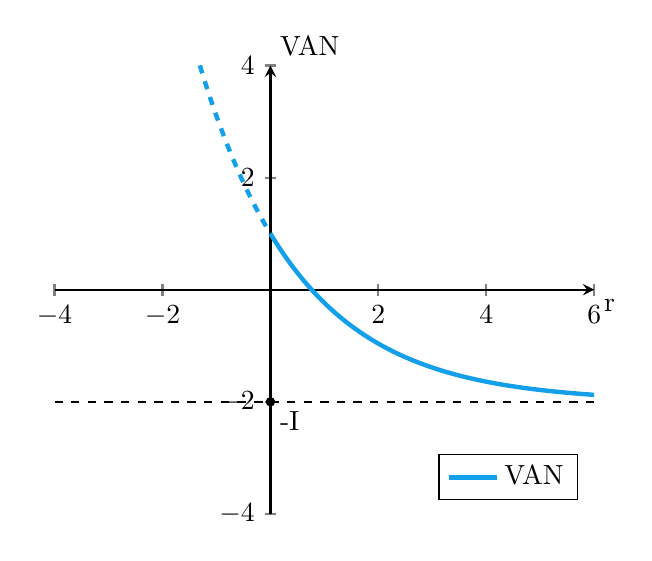
\begin{tikzpicture}[scale = 1,
            declare function={
                    f(\x) = 3/((1+0.7)^(\x)) -2;
                    g(\x) = -2;
                }]
        \def\p{0.76}
        \begin{axis}
            [
                xlabel={\( \text{r} \)},
                ylabel={\( \text{VAN} \)},
                xmin=-4, xmax=6,
                ymin=-4, ymax=4,
                grid=both,
                grid=none, axis lines=middle, 
                axis line style={-stealth, thick},
                tick style={thick},
                xlabel style={at={(ticklabel* cs:1)}, anchor=north west},
                ylabel style={at={(ticklabel* cs:1)}, anchor=south west},
                samples=100, unbounded coords=jump, legend pos=south east
            ]
            \addplot [domain=0: 6, ultra thick, smooth, color=myblue]{f(x)};
            \addplot [domain=-4: 0, ultra thick, dashed, color=myblue]{f(x)};
            \addplot [domain=-4: 6, thick , dashed]{g(x)};
            \node [below right] at (axis cs: 0, -2) {-I};
            \filldraw (axis cs:0,-2) circle (1.5pt);
            \legend{VAN}
        \end{axis}
    \end{tikzpicture}
\end{document}